\documentclass[12pt,fleqn]{article}

\usepackage{graphicx}
\usepackage{paralist}
\usepackage{amsfonts}
\usepackage{graphicx}

\oddsidemargin 0mm
\evensidemargin 0mm
\textwidth 180mm
\textheight 200mm
\renewcommand\baselinestretch{1.0}

\pagestyle {plain}
\pagenumbering{arabic}

\newcounter{stepnum}

\title{Software Specifications Document \\ReLocate\\version 3.2}

\author{COMP SCI 2XB3\\  
Computer Science Practice and Experience: Binding Theory to Practice\\ \\ \\
Group 04\\Madeeha Khan, Tasnim Noshin, Umme Salma Gadriwala,\\ 
Jenny Feng Chen, Patrick Laskowski \\ \\ \\
Department of Computer Science\\ 
McMaster University}

\begin {document}

\maketitle

\newpage
\section*{Revisions}\label{revisions}

%%%%%%%%%%%%%%%%%%%%%%%%%%%%%%%%%%%%%%%%%%%%%%%%%%%%%%%%%%%%%%%%%%%%%%


\newpage
\section*{Contributions}\label{contributions}


%%%%%%%%%%%%%%%%%%%%%%%%%%%%%%%%%%%%%%%%%%%%%%%%%%%%%%%%%%%%%%%%%%%%%%


\newpage
\section*{Executive Summary}


%%%%%%%%%%%%%%%%%%%%%%%%%%%%%%%%%%%%%%%%%%%%%%%%%%%%%%%%%%%%%%%%%%%%%%

\newpage
\section*{Module Decomposition}

\begin{figure}[hp!]
\caption{UML class diagram with relations. Figure is only visible from 250\%+ zoom}
  \hspace*{-4.4cm}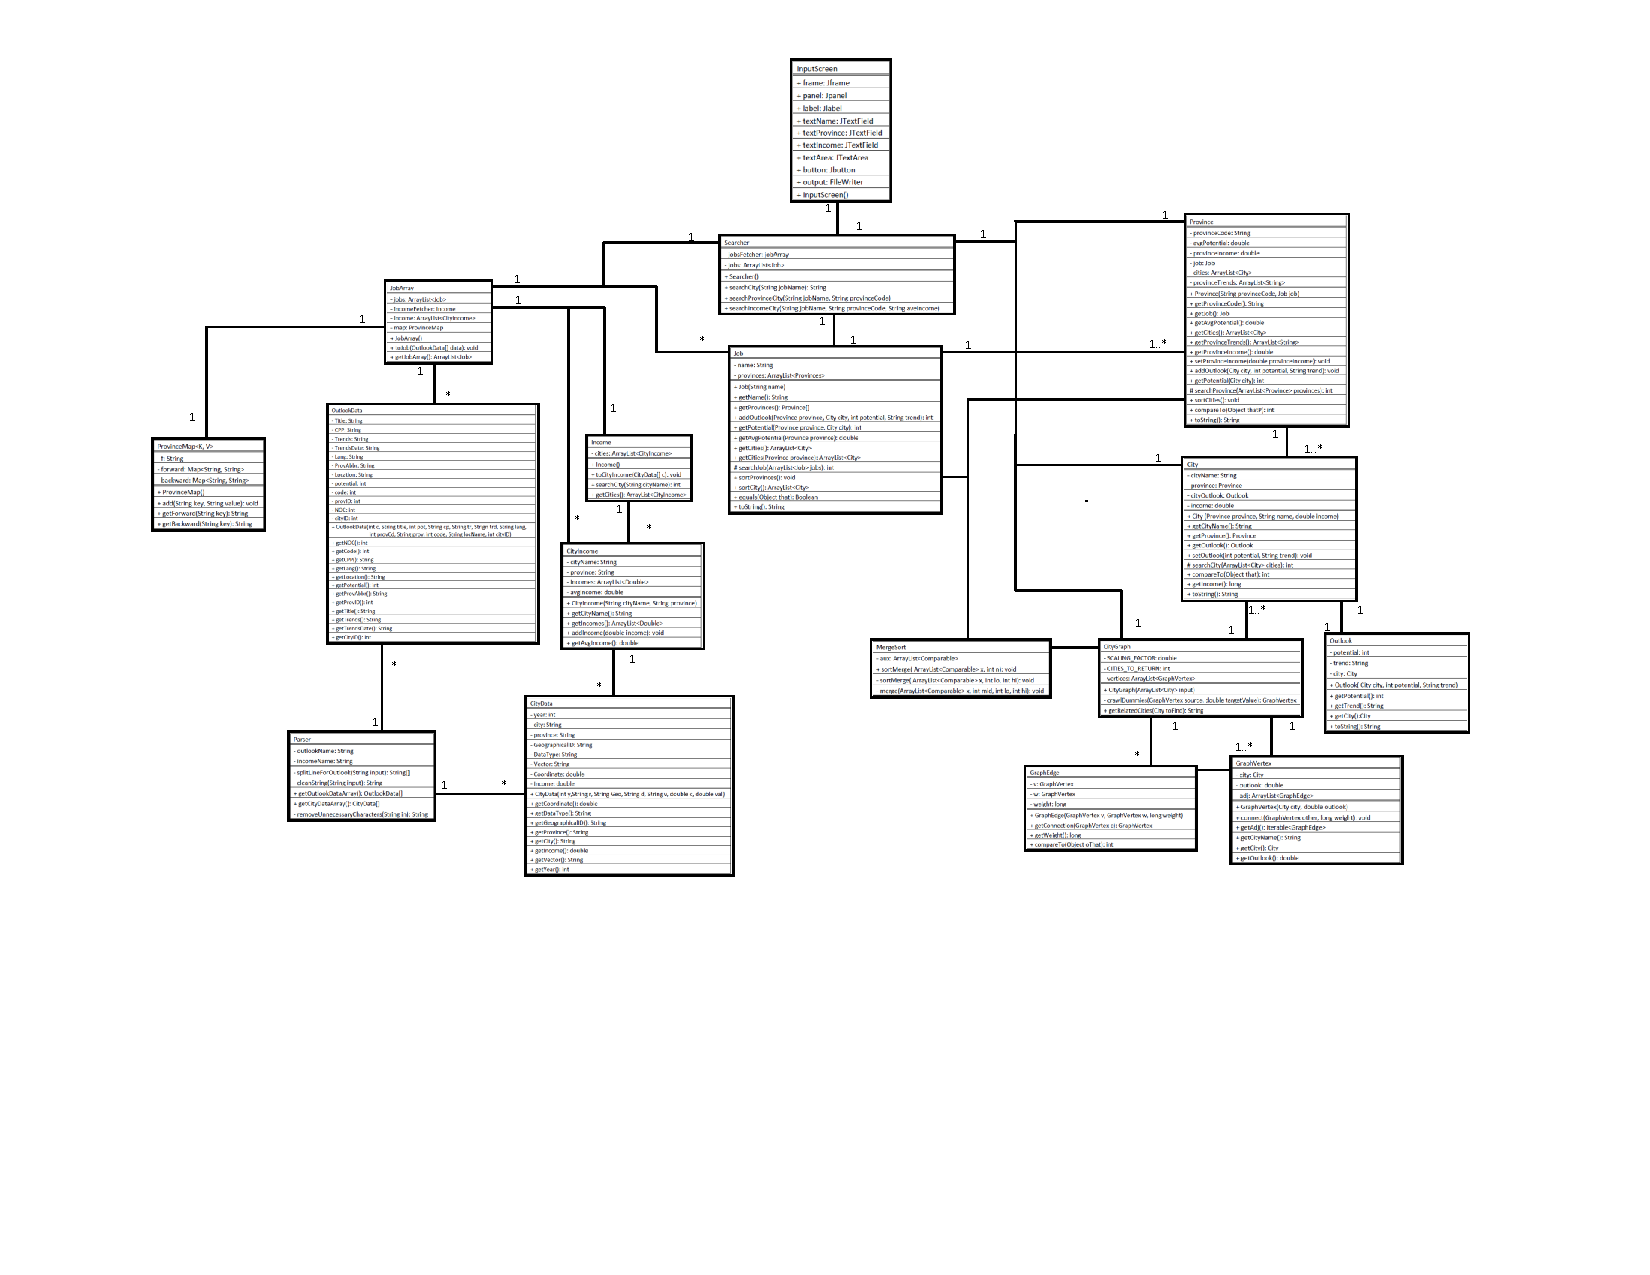
\includegraphics[width = 260mm]{Group04_Classes_Diagram.pdf}
\end{figure}


%%%%%%%%%%%%%%%%%%%%%%%%%%%%%%%%%%%%%%%%%%%%%%%%%%%%%%%%%%%%%%%%%%%%%%


\newpage
\section*{Public Methods Description}\label{public}
\subsection*{City.java}\label{city}
This class represents a city.
\subsubsection* {Syntax}

\subsubsection* {Access Programs}
\begin{tabular}{| l | l | l | l |}
\hline
\textbf{Routine name} & \textbf{Input} & \textbf{Output} & \textbf{Exceptions}\\
\hline
City & Province, String, Double & City & ~\\
\hline
getCityName & ~ & String & ~\\
\hline
getProvince & ~ & Province & ~\\
\hline
getOutlook & ~ & Outlook & ~\\
\hline
setOutlook & int, String & ~ & ~\\
\hline
searchCity & ArrayList$<$City$>$ & int & ~\\
\hline
toString & ~ & String & ~\\
\hline
compareTo & Object & int & ~\\
\hline
\end{tabular}

\subsubsection*{Semantics}
\subsubsection*{Access Routine Semantics}
\noindent City($province, name, income$)
\begin{itemize}
\item This is a constructor that takes a province object, a city name and a median income of the city as inputs
and assigns them to each of the field in city.
\end{itemize}
\noindent getCityName()
\begin{itemize}
\item This method returns the city name.
\end{itemize}
\noindent getProvince()
\begin{itemize}
\item This method returns the province object.
\end{itemize}
\noindent getOutlook()
\begin{itemize}
\item This method returns the outlook of the city.
\end{itemize}
\noindent setOutlook()
\begin{itemize}
\item This method set the outlook of the city.
\end{itemize}
\noindent searchCity($cities$)
\begin{itemize}
\item This method search the city in the given list of cities.
\\Returns the index of the city in the list if found else returns -1.
\end{itemize}
\noindent toString()
\begin{itemize}
\item Returns the representation of the city as string.
\end{itemize}
\noindent compareTo($thatC$)
\begin{itemize}
\item If the values of outlook of the two objects are equal return 0. If the value of outlook of this object is
greater than the weight of the given object return 1, else return -1.
\end{itemize}

%%%%%%%%%%%%%%%%%%%%%

\subsection*{CityData.java}\label{cityd}
This class represents a city with corresponding data from dataset of income.
\subsubsection* {Syntax}

\subsubsection* {Access Programs}
\begin{tabular}{| l | l | l | l |}
\hline
\textbf{Routine name} & \textbf{Input} & \textbf{Output} & \textbf{Exceptions}\\
\hline
CityData & int, String, String, String, String, double, double & CityData & ~\\
\hline
 getCoordinate& ~ & double & ~\\
\hline
getDataType & ~ & String & ~\\
\hline
getGeographicalID & ~ & String & ~\\
\hline
getProvince & ~ & String & ~\\
\hline
getCity & ~ & String & ~\\
\hline
getIncome & ~ & double & ~\\
\hline
getVector & ~ & String & ~\\
\hline
getYear & ~ & int & ~\\

\hline
\end{tabular}

\subsubsection*{Semantics}
\subsubsection*{Access Routine Semantics}
\noindent CityData($y, r, Geo, d, v, c, val$)
\begin{itemize}
\item This constructor takes a year, city name, province name, geographical ID, data type, vector, coordinates
and income to assign each field of the CityData object.
\end{itemize}
\noindent getCoordinate()
\begin{itemize}
\item Returns the coordinate value of the data.
\end{itemize}
\noindent getDataType()
\begin{itemize}
\item Returns the type of the data as string.
\end{itemize}
\noindent getGeographicalID()
\begin{itemize}
\item Returns the Geographical ID as string.
\end{itemize}
\noindent getProvince()
\begin{itemize}
\item Returns the province name where the data was collected in.
\end{itemize}
\noindent getCity()
\begin{itemize}
\item Returns the city name where the data was collected in.
\end{itemize}
\noindent getIncome()
\begin{itemize}
\item Returns the income of the data.
\end{itemize}
\noindent getVector()
\begin{itemize}
\item Returns the vector representation as string.
\end{itemize}
\noindent getYear()
\begin{itemize}
\item Returns an integer holding the year the data was collected in.
\end{itemize}

%%%%%%%%%%%%%%%%%%%%%

\subsection*{CityGraph.java}\label{graph}
This class is used to create the actual undirected graph of the city.
\subsubsection* {Syntax}

\subsubsection* {Access Programs}
\begin{tabular}{| l | l | l | l |}
\hline
\textbf{Routine name} & \textbf{Input} & \textbf{Output} & \textbf{Exceptions}\\
\hline
 CityGraph& ArrayList$<$City$>$ & CityGraph & ~\\
\hline
getRelatedCities & City & String & ~\\
\hline
getRelatedCitiesTest & City & ArrayList$<$City$>$& ~\\
\hline
\end{tabular}

\subsubsection*{Semantics}
\subsubsection*{Access Routine Semantics}
\noindent CityGraph($input$)
\begin{itemize}
\item This constructor takes an arrayList of type City to make the graph.\\
Add all cities into the graph in the proper place by creating a new vertex to represent a city in the
arraylist and add it to the graph. Then link each vertex to the correct vertex with income as the weight.
\end{itemize}
\noindent getRelatedCities($toFind$)
\begin{itemize}
\item This method takes a City object and returns a few cities related to the given City object.\\
Scan for the given city as vertex in the graph if not null, and if there are adjacent vertices for the given
city hold the vertex else return null. If a vertex is hold, put all the edges into an arrayList excluding the
original city. Sort the arrayList using merge sort by edges weight.
Returns the sorted arrayList of cities as String.
\end{itemize}
\noindent getRelatedCitiesTest($toFind$)
\begin{itemize}
\item This is a reduced version of the above function that is used for testing, and does essentailly the same, except it returns the ArrayList instead of its String represenation
\end{itemize}

%%%%%%%%%%%%%%%%%%%%%

\subsection*{CityIncome.java}\label{cityincome}
This class represents a city with income from the income dataset.
\subsubsection* {Syntax}

\subsubsection* {Access Programs}
\begin{tabular}{| l | l | l | l |}
\hline
\textbf{Routine name} & \textbf{Input} & \textbf{Output} & \textbf{Exceptions}\\
\hline
CityIncome & String, String & CityIncome & ~\\
\hline
getCityName & ~ & String & ~\\
\hline
getIncome & ~ & ArrayList$<$Souble$>$ & ~\\
\hline
addIncome & double & ~ & ~\\
\hline
getAvgIncome & ~ & double & ~\\
\hline
\end{tabular}

\subsubsection*{Semantics}
\subsubsection*{Access Routine Semantics}
\noindent CityIncome($cityName, province$)
\begin{itemize}
\item This constructor takes a city name and the province name which to assign for the city and province. It
initializes an empty arraylist of type double for income and sets the average income as 0.
\end{itemize}
\noindent getCityName()
\begin{itemize}
\item Returns the city name.
\end{itemize}
\noindent getIncome()
\begin{itemize}
\item Returns an arrayList of income of type double.
\end{itemize}
\noindent addIncome($income$)
\begin{itemize}
\item Takes an income and adds to the arrayList of income of the city and updates the average income of the
city.
\end{itemize}
\noindent getAvgIncome()
\begin{itemize}
\item Returns the average income of the city.
\end{itemize}

%%%%%%%%%%%%%%%%%%%%%

\subsection*{GraphEdge.java}\label{edge}
This class is used as an edge to connect two vertices.
\subsubsection* {Syntax}

\subsubsection* {Access Programs}
\begin{tabular}{| l | l | l | l |}
\hline
\textbf{Routine name} & \textbf{Input} & \textbf{Output} & \textbf{Exceptions}\\
\hline
GraphEdge & GraphVertex, GraphVertex, double & ~ & ~\\
\hline
getConnection & GraphVertex & GraphVertex & ~\\
\hline
getWeight & ~ & long & ~\\
\hline
compareTo & Object & int & ~\\
\hline
\end{tabular}

\subsubsection*{Semantics}
\subsubsection*{Access Routine Semantics}
\noindent GraphEdge($v, w, weight$)
\begin{itemize}
\item This method takes two GraphVertex object and a double for the weight to constructs a GraphEdge by
assigning them the corresponding value to the corresponding fields.
\end{itemize}
\noindent getConnection($c$)
\begin{itemize}
\item It takes a GraphVertex object and checks whether the object is equal to either of the GraphVertex in the
filed if not, returns null else return the the one that is equal.
\end{itemize}
\noindent getWeight()
\begin{itemize}
\item Return the weight of this edge as double.
\end{itemize}
\noindent compareTo($that$)
\begin{itemize}
\item If the weights of the two objects are equal return 0. If the weight of this object is greater than the weight
of the given object return 1, else return -1.
\end{itemize}

%%%%%%%%%%%%%%%%%%%%%

\subsection*{GraphVertex.java}\label{vertex}
This class represents a vertex as a city, with its outlook and its adjacent vertices
\subsubsection* {Syntax}

\subsubsection* {Access Programs}
\begin{tabular}{| l | l | l | l |}
\hline
\textbf{Routine name} & \textbf{Input} & \textbf{Output} & \textbf{Exceptions}\\
\hline
GraphVertex & City, double & GraphVertex & ~\\
\hline
connect & GraphVertex, long & ~ & ~\\
\hline
getAdj & ~ & Iterable$<$GraphEdge$>$ & ~\\
\hline
getCityName & ~ & String & ~\\
\hline
getCity & ~ & City & ~\\
\hline
getOutlook & ~ & double & ~\\
\hline
\end{tabular}

\subsubsection*{Semantics}
\subsubsection*{Access Routine Semantics}

%%%%%%%%%%%%%%%%%%%%%

\subsection*{Income.java}\label{income}
This class holds an arrayList of type CityIncome.
\subsubsection* {Syntax}

\subsubsection* {Access Programs}
\begin{tabular}{| l | l | l | l |}
\hline
\textbf{Routine name} & \textbf{Input} & \textbf{Output} & \textbf{Exceptions}\\
\hline
Income & ~ & Income& ~\\
\hline
toCityIncome & CityData[] & ~ & ~\\
\hline
searchCity & String & int & ~\\
\hline
getCities & ~ & ArrayList$<$CityIncome$>$ & ~\\
\hline
\end{tabular}

\subsubsection*{Semantics}
\subsubsection*{Access Routine Semantics}
\noindent Income()
\begin{itemize}
\item Initializes an empty arrayList and creates a CityData array from the parser of CityData. Constructs the
arrayList of CityIncome by converting the CityData array to arrayList of CityIncome. Thorws IOException
when getting data from the Parser.
\end{itemize}
\noindent toCityIncome($c$)
\begin{itemize}
\item For every city in $c$, it creates a new CityIncome object with that city's City and Province fields.
\\if the city did not already exist in the array c, it adds the income to the city, and adds the city to the cities
\\otherwise, it adds the income to the already existing city.
\\If there is no city, and only a province,  it creates a City and adds it at the end of the ArrayList
\end{itemize}
\noindent searchCity($cityName$)
\begin{itemize}
\item Takes a city name and search for the city in the arrayList of the CityIncome. Returns -2 if input is null,
returns the index where the city name is in the arraylist if found, else return -1 where city name is valid
but not found in the arraylist.
\end{itemize}
\noindent getCities()
\begin{itemize}
\item Return the arrayList of type CityIncome
\end{itemize}

%%%%%%%%%%%%%%%%%%%%%

\subsection*{InputScreen.java}\label{input}
This class represents the GUI, where the user can enter the information they wish to find through the job search.
\subsubsection* {Syntax}

\subsubsection* {Access Programs}
\begin{tabular}{| l | l | l | l |}
\hline
\textbf{Routine name} & \textbf{Input} & \textbf{Output} & \textbf{Exceptions}\\
\hline
InputScreen & ~ & ~ & IOException\\
\hline
\end{tabular}

\subsubsection*{Semantics}
\subsubsection*{Access Routine Semantics}
\noindent InputScreen()
\begin{itemize}
\item Constructor, which creates the JFrame with all the labels, panels, and buttons in it, and also keeps track
of the actions (entering texts and pushing the button). The constructor is also where the search is
performed and the results are written into the output file for the user.\\
The search is performed by calling the methods from the Searcher class, depending on what the input is
from the user:
\begin{itemize}
\item If just a job name is given, the searchCity method is called on the job name given
\item If a job name and a province are given, the searchProvinceCity method is called on them
\item If all three are specified, the searchIncomeCity method is called on them
\item If an invalid combination (no job name, only a job name and an income), a “not found” message
is displayed
\end{itemize}
There is an IOException thrown if there is an issue with the output file for whatever reason.
\end{itemize}

%%%%%%%%%%%%%%%%%%%%%

\subsection*{Job.java}\label{job}
This is the class representing a job. 
\subsubsection* {Syntax}

\subsubsection* {Access Programs}
\begin{tabular}{| l | l | l | l |}
\hline
\textbf{Routine name} & \textbf{Input} & \textbf{Output} & \textbf{Exceptions}\\
\hline
Job & String & Job & ~\\
\hline
getName & ~ & String & ~\\
\hline
getProvinces & ~ & Provinces[] & ~\\
\hline
addOutlook & Province, City, int, String & ~  & ~\\
\hline
getPotential & Province, City & int & ~\\
\hline
getAvgPotential & Province & double & ~\\
\hline
getCities & ~ & ArrayList$<$City$>$ & ~\\
\hline
getCities & Province &  ArrayList$<$City$>$ & ~\\
\hline
searchJob &ArrayList$<$Job$>$  & int & ~\\
\hline
sortProvinces & ~ & ~ & ~\\
\hline
sortCity & ~ & ArrayList$<$City$>$ & ~\\
\hline
equals & Object & boolean & ~\\
\hline
toString & ~ & String & ~\\
\hline
\end{tabular}

\subsubsection*{Semantics}
\subsubsection*{Access Routine Semantics}
\noindent Job()
\begin{itemize}
\item The constructor, which takes a string (the name of the job), and creates an ArrayList of type Province to
hold all the provinces the job is found in.
\end{itemize}
\noindent getName()
\begin{itemize}
\item returns the String, name of the job
\end{itemize}
\noindent getProvinces()
\begin{itemize}
\item returns an array of Provinces
\end{itemize}
\noindent addOutlook($province, city, potential, trend$)
\begin{itemize}
\item the spot of the province is found in this.provinces (through a for-loop in the Provinces class)
an outlook is added (called from the Province class) in that spot for that province if it exists in the
arrayList
\\if the province is not found in the list of provinces for that job (index = -1), it is added to the end of the
list and an outlook is given to it (called from the Province class)
\end{itemize}
\noindent getPotential($province, city$)
\begin{itemize}
\item the spot of the specified province is searched in this.provinces (from the Province class, in a for-loop)
if the province is in the list, it finds the province in the list and gets the potential for the city in that
province\\
if the province is not in the list of provinces (index = -1), 0 is returned (since it means undetermined)
\end{itemize}
\noindent getAvgPotential($province$)
\begin{itemize}
\item gets the average potential for that province if the province is in this.provinces
otherwise, returns 0
\end{itemize}
\noindent getCities()
\begin{itemize}
\item returns all the cities that the job is in
\end{itemize}
\noindent getCities($province$)
\begin{itemize}
\item returns all the cities the job is in, in a given province
\end{itemize}
\noindent searchJob($jobs$)
\begin{itemize}
\item find the index of a job in the ArrayList of jobs by looping through the list and checking if the name of the
job is in the list
\end{itemize}
\noindent sortProvinces()
\begin{itemize}
\item sorts the provinces the job is in according to the avgPotential with Mergesort
\end{itemize}
\noindent sortCity()
\begin{itemize}
\item sort the cities the job is in according to their potentials with Mergesort
\end{itemize}
\noindent equals($that$)
\begin{itemize}
\item checks if 2 jobs are equal by first checking if they are of the same Class, then uses the built-in euqals
method to check their equality
\end{itemize}
\noindent toString()
\begin{itemize}
\item returns a String representation of the Job object, which includes the name and all the provinces it is in
\end{itemize}

%%%%%%%%%%%%%%%%%%%%%

\subsection*{JobArray.java}\label{jobarray}
This class creates the array of Jobs that will later be searched to match a job inputted by the user and find its information.
\subsubsection* {Syntax}

\subsubsection* {Access Programs}
\begin{tabular}{| l | l | l | l |}
\hline
\textbf{Routine name} & \textbf{Input} & \textbf{Output} & \textbf{Exceptions}\\
\hline
JobArray & ~ & JobArray & IOException\\
\hline
toJob & OutlookData[] & ~ & ~\\
\hline
getJobArray & ~ & ArrayList$<$Job$>$ & ~\\
\hline
\end{tabular}

\subsubsection*{Semantics}
\subsubsection*{Access Routine Semantics}
\noindent JobArray()
\begin{itemize}
\item The constructor initiliazes the instance variables, and also grabs an array of OutlookData[] from the Parser, which has scraped the csv file. It then takes this arrya and turns every entry in it into an instance of the Job class with the toJob method.
\end{itemize}
\noindent toJob($data$)
\begin{itemize}
\item this method takes the OutlookData[] array from the constructor and for every entry $od$ in the array, creates a new job with $od$'s title, and checks to see if the job already exists in the array
\\If it does not, it gets the name of the province(s) that the job exists in from the ProvinceMap (the key is the abbreviation of $od$'s province from the csv file), then it finds the income of the cities that the job is in, as well as the avergae income for the province, and adds cities and outlook information for the job. The job is then added to the end of the array.
\\If the job already existed in the array, it finds that job's position in the array, then adds all of the same information as above.
\end{itemize}
\noindent getJobArray()
\begin{itemize}
\item returns the job array
\end{itemize}

%%%%%%%%%%%%%%%%%%%%%

\subsection*{MergeSort.java}\label{sort}
This class sorts an arrayList where extends the comparable type.
\subsubsection* {Syntax}

\subsubsection* {Access Programs}
\begin{tabular}{| l | l | l | l |}
\hline
\textbf{Routine name} & \textbf{Input} & \textbf{Output} & \textbf{Exceptions}\\
\hline
sortMerge & ArrayList$<$Comparable$>$, int & ~ & ~\\
\hline
\end{tabular}

\subsubsection*{Semantics}
\subsubsection*{Access Routine Semantics}
\noindent sortMerge($x, n$)
\begin{itemize}
\item This method takes an arrayList of Comparable type and the size of arrayList. It constructs an arrayList of
the same size with each of the element initializing to null. Then merge sort the list.
\end{itemize}

%%%%%%%%%%%%%%%%%%%%%

\subsection*{Outlook.java}\label{outlook}
This class gives the outlook for a City, which is the combination of its potential and its trend.
\subsubsection* {Syntax}

\subsubsection* {Access Programs}
\begin{tabular}{| l | l | l | l |}
\hline
\textbf{Routine name} & \textbf{Input} & \textbf{Output} & \textbf{Exceptions}\\
\hline
Outlook & City, int, String & Outlook & ~\\
\hline
getPotential & ~ & int & ~\\
\hline
getTrend & ~ & String & ~\\
\hline
getCity & ~ & City & ~\\
\hline
toString & ~ & String & ~\\
\hline
\end{tabular}

\subsubsection*{Semantics}
\subsubsection*{Access Routine Semantics}
\noindent Outlook($city, potential, trend$)
\begin{itemize}
\item this constructor initilizaes the instance variables to the given arguments to create a new instance of the Outlook class
\end{itemize}
\noindent getPotential()
\begin{itemize}
\item returns the int $potential$
\end{itemize}
\noindent getTrend()
\begin{itemize}
\item returns the String $trend$
\end{itemize}
\noindent getCity()
\begin{itemize}
\item returns the City object $city$
\end{itemize}
\noindent toString()
\begin{itemize}
\item returns a string representation of each Outlook object, with its potential, and trend.
\end{itemize}

%%%%%%%%%%%%%%%%%%%%%

\subsection*{OutlookData.java}\label{outlookd}
This is the info scraped from the outlooks.csv file. Each instance of his class represents a line from that file.
\subsubsection* {Syntax}

\subsubsection* {Access Programs}
\begin{tabular}{| l | l | l | l |}
\hline
\textbf{Routine name} & \textbf{Input} & \textbf{Output} & \textbf{Exceptions}\\
\hline
OutlookData & int, String, int, String, String, String, \\&String,  int, String, int, String, int & OutlookData & ~\\
\hline
getNOC & ~ & int & ~\\
\hline
getCode & ~ & int & ~\\
\hline
getCPP & ~ & String & ~\\
\hline
getLang & ~ & String & ~\\
\hline
getLocation & ~ & String & ~\\
\hline
getPotential & ~ & int & ~\\
\hline
getProvAbbr & ~ & String & ~\\
\hline
getProvID & ~ & int & ~\\
\hline
getTitle & ~ & String & ~\\
\hline
getTrends & ~ & String & ~\\
\hline
getTrendsDate & ~ & String& ~\\
\hline
getCityID & ~ & int & ~\\
\hline
\end{tabular}

\subsubsection*{Semantics}
\subsubsection*{Access Routine Semantics}
\noindent OutlookData ($c, title, pot, cp, tr, trd, lang, provCd, prov, code, locName , cityID$)
\begin{itemize}
\item The constructor creates a new instance of OutlookData by taking the given arguments and assigning them to instance variables. 
\\If the locName is the name of a province, it is nulled out, since we want that information for cities only.
\end{itemize}
\noindent getNoc()
\begin{itemize}
\item returns the int $NOC$
\end{itemize}
\noindent getCode()
\begin{itemize}
\item returns the int $code$
\end{itemize}
\noindent getCPP()
\begin{itemize}
\item returns the String $CPP$
\end{itemize}
\noindent getLang()
\begin{itemize}
\item returns the String $lang$
\end{itemize}
\noindent getLocation()
\begin{itemize}
\item returns the String $location$
\end{itemize}
\noindent getPotential()
\begin{itemize}
\item returns the int $potential$
\end{itemize}
\noindent getProvAbbr()
\begin{itemize}
\item return the String $provAbbr$
\end{itemize}
\noindent getProvID()
\begin{itemize}
\item returns the int $provID$
\end{itemize}
\noindent getTitle()
\begin{itemize}
\item returns the String $title$
\end{itemize}
\noindent getTrends()
\begin{itemize}
\item returns the String $trends$
\end{itemize}
\noindent getTrendsDate()
\begin{itemize}
\item returns th String $trendsDate$
\end{itemize}
\noindent getCityID()
\begin{itemize}
\item returns int $cityID$
\end{itemize}

%%%%%%%%%%%%%%%%%%%%%

\subsection*{Parser.java}\label{p
arser}
This class takes the outlooks.csv and income.csv files and scrapes them, and creates arrays out of their information.
\subsubsection* {Syntax}

\subsubsection* {Access Programs}
\begin{tabular}{| l | l | l | l |}
\hline
\textbf{Routine name} & \textbf{Input} & \textbf{Output} & \textbf{Exceptions}\\
\hline
getOutlookDataArray & ~ & OutlookData[] & IOException\\
\hline
getCityDataArray & ~ & CityData[] & IOException\\
\hline
\end{tabular}

\subsubsection*{Semantics}
\subsubsection*{Access Routine Semantics}
\noindent getOutlookDataArray()
\begin{itemize}
\item This method scrapes the outlooks.csv file and for each entry creates a new object of class OutlookData, then stores them in an array to be returned.
\\It reads each line of the csv file (skipping the first line, since it has the headings), and intializes an array to the size of number of lines in the file. Then, it takes each row in the file and splits them with a private method to create the fields of an OutlookData object, and creates new objects with those fields.
\end{itemize}
\noindent getCity DataArray()
\begin{itemize}
\item This method scrapes the incomes.csv file and for each entry creates a new object of class CityData, then stores them in an array to be returned.
\\First, an array is created to the size of number of lines in the file. Then, each row in the file is split and its components are used as arguments to create new CityData objects, which are then stored in the array.
\\this method deals with blank lines and fills in '0' for them, as well as inappropriate types (if the file provides a String instead of an int, it is given an error value of int -1).
\end{itemize}

%%%%%%%%%%%%%%%%%%%%%

\subsection*{Province.java}\label{prov}
This class represents a province, and contains all the information available about provinces from the combination of both datasets
\subsubsection* {Syntax}

\subsubsection* {Access Programs}
\begin{tabular}{| l | l | l | l |}
\hline
\textbf{Routine name} & \textbf{Input} & \textbf{Output} & \textbf{Exceptions}\\
\hline
Province & String, Job & Province & ~\\
\hline
 getProvinceCode& ~ & String & ~\\
\hline
getJob & ~ & Job & ~\\
\hline
getAvgPotential & ~ & double & ~\\
\hline
getCities & ~ & ArrayList$<$City$>$ & ~\\
\hline
getProvinceTrends & ~ &  ArrayList$<$String$>$ & ~\\
\hline
getProvinceName & ~ & double & ~\\
\hline
getProvinceIncome & ~ & double & ~\\
\hline
addOutlook & City, int, String & ~ & ~\\
\hline
getPotential & City & int & ~\\
\hline
SearchProvince & ArrayList$<$Province$>$ & int & ~\\
\hline
sortCities & ~ & ~ & ~\\
\hline
compareTo & Object & int & ~\\
\hline
toString & ~ & String & ~\\
\hline
setProvinceIncome & ~ & double & ~\\
\hline
\end{tabular}

\subsubsection*{Semantics}
\subsubsection*{Access Routine Semantics}
\noindent Province($provinceCode, job$)
\begin{itemize}
\item This constructor initializes all the instance variables to create a new Province object
\end{itemize}
\noindent getProvinceCode()
\begin{itemize}
\item returns  String $provinceCode$
\end{itemize}
\noindent getJob()
\begin{itemize}
\item returns Job object $job$
\end{itemize}
\noindent getAvgPotential()
\begin{itemize}
\item returns double $avgPotential$
\end{itemize}
\noindent getCities()
\begin{itemize}
\item returns ArrayList$<$City$>$ $cities$
\end{itemize}
\noindent getProvinceTrends()
\begin{itemize}
\item returns ArrayList$<$String$>$ $provinceTrends$
\end{itemize}
\noindent getProvinceName()
\begin{itemize}
\item returns double $provinceName$
\end{itemize}
\noindent getProvinceIncome()
\begin{itemize}
\item returns double $provinceIncome$
\end{itemize}
\noindent addOutlook($city, potential, trend$)
\begin{itemize}
\item takes a $city, potential, trend$ tuple and 
\\if the $city$ name is null, it adds the trend to the end of the $provinceTrends$.
\\Otherwise, it finds $city$ in $cities$ and if the city does not already exist, it creates an outlook for the city with the $trend$ and $potential$, and adds it to $cities$. 
\\If the city already exists, it gets the city at the index that matches $city$ in $cities$, gives it the $potential$ and $trend$, and puts it in $cities$ at the same index.
\end{itemize}
\noindent getPotential($city$)
\begin{itemize}
\item This method finds $city$ in $cities$ and returns 0 if $city$ is not there, returns the potential for $city$ if it is.
\end{itemize}
\noindent searchProvince(provinces)
\begin{itemize}
\item For every province in $provinces$, it tried to match $provinceCode$ to the entry in the ArrayList, and returns the index of it if it is found, and -1 if it is not.
\end{itemize}
\noindent sortCities()
\begin{itemize}
\item This method uses MergeSort to sort the $cities$ by their potentials.
\end{itemize}
\noindent compareTo($that$)
\begin{itemize}
\item Compares two Provinces byt their potentials, returns:
\begin{itemize}
\item 2 if $this$ and $that$ are not provinces for the same job.
\item 1 if $this$'s potential is larger
\item 0 if they have equal potentials
\item -1 if $that$'s potential is larger
\end{itemize}
\end{itemize}
\noindent toString()
\begin{itemize}
\item Returns a String representation of the Province, with all its cities, provinceCode, average Potential, and provincial trends.
\end{itemize}
\noindent setProvinceIncome($provinceIncome$)
\begin{itemize}
\item Sets the income to the specified value.
\end{itemize}

%%%%%%%%%%%%%%%%%%%%%

\subsection*{ProvinceMap.java}\label{provmap}
This class holds two maps which the key of one map is province name and value is the abbreviation
whereas the other map’s key is abbreviation and value is province name.
\subsubsection* {Syntax}

\subsubsection* {Access Programs}
\begin{tabular}{| l | l | l | l |}
\hline
\textbf{Routine name} & \textbf{Input} & \textbf{Output} & \textbf{Exceptions}\\
\hline
ProvinceMap & ~ & ~ & FileNotFoundException\\
\hline
add & String, String & ~ & ~\\
\hline
getForward & String & String & ~\\
\hline
getBackward & String & String & ~\\
\hline
\end{tabular}

\subsubsection*{Semantics}
\subsubsection*{Access Routine Semantics}
\noindent ProvinceMap()
\begin{itemize}
\item Scan the file containing provinces and abbreviation and store the data into two maps.\\Each line consists of
a province name and an abbreviation, split them by a comma. 
\end{itemize}
\noindent add($key, value$)
\begin{itemize}
\item add the key and the value to each of the map
\end{itemize}
\noindent getCityAbbr($key$)
\begin{itemize}
\item This method takes a string of province name and returns the corresponding abbreviation.
\end{itemize}
\noindent getCityName($key$)
\begin{itemize}
\item This method takes a string of abbreviation and returns the corresponding province name.
\end{itemize}

%%%%%%%%%%%%%%%%%%%%%

\subsection*{Searcher.java}\label{search}
This class is where the searching happens. It has different methods for different kinds of searches, depending on what information the user gives, and also has reduced versions of the methods for testing. It throws an IOException because it has cennections to the Parser, which uses files.
\subsubsection* {Syntax}

\subsubsection* {Access Programs}
\begin{tabular}{| l | l | l | l |}
\hline
\textbf{Routine name} & \textbf{Input} & \textbf{Output} & \textbf{Exceptions}\\
\hline
Searcher & ~ & Searcher & IOException\\
\hline
searchCity & String & String & IOException\\
\hline
searchProvinceCity & String, String & String& IOException\\
\hline
searchIncomeCity & String, String, String & String & IOException\\
\hline
searchCityTest & String & int & IOException\\
\hline
searchProvinceCityTest & String, String & ArrayList$<$City$>$ & IOException\\
\hline
searchIncomeProvinceTest & String, String, String & ArrayList$<$City$>$ & IOException\\
\hline
\end{tabular}

\subsubsection*{Semantics}
\subsubsection*{Access Routine Semantics}
\noindent searchCity($jobName$)
\begin{itemize}
\item This method searches through the job array when the name of a job is given.
\\it creates a new JobArray, then finds the index of the entry whose name matches $jobName$. If the job is not there, it will give -1, and the message "Job not found" is returned. 
\\An ArrayList of type City is created, where the cities that have the job in them are put, then sorted by their potential. Each entry in this list is then turned into its String representation and added to the result string. When all the cities have been added, the String is returned.
\end{itemize}
\noindent searchProvinceCity($jobName, provinceCode$)
\begin{itemize}
\item This method performs the same function as above, but only adds the city to the result String if its provinceCode matches the city's. Returns the first 5 things in the ArrayList, in String form.
\end{itemize}
\noindent searchIncomeCity($jobName, provinceCode, aveIncome$)
\begin{itemize}
\item This method takes a String $aveIncome$ and parses it to a double, then performs the same function as the method above, except the city is only added to the result String if the income is equal to or above the specified $aveIncome$. The result String is the first 5 entries in the ArrayList in String form.
\end{itemize}
\noindent searchCityTest($jobName$)
\begin{itemize}
\item This method was created for testing searchCity($jobname$). It returns the index of the job instead of its String representation.
\end{itemize}
\noindent searchProvinceCityTest($jobname, provinceCode$)
\begin{itemize}
\item This method was created for testing searchProvinceCity($jobname, provinceCode$). It returns the sorted ArrayList instead of its String representation.
\\It would return an empty ArrayList if the job did not exist.
\end{itemize}
\noindent searchIncomeCity($jobname, provinceCode, aveIncome$)
\begin{itemize}
\item This method was created for testing searchIncomeCity($jobname, provinceCode, aveIncome$). It returns the sorted ArrayList instead of its String representation.
\\It would return an empty ArrayList if the job did not exist.
\end{itemize}

%%%%%%%%%%%%%%%%%%%%%

\subsection*{TestGraph.java}\label{testg}
This class tests the CityGraph and takes its input from a text file testText.txt
\subsubsection* {Syntax}

\subsubsection* {Access Programs}
\begin{tabular}{| l | l | l | l |}
\hline
\textbf{Routine name} & \textbf{Input} & \textbf{Output} & \textbf{Exceptions}\\
\hline
test & ~ & ~ & IOException\\
\hline
\end{tabular}

\subsubsection*{Semantics}
\subsubsection*{Access Routine Semantics}
\noindent test()
\begin{itemize}
\item This method tests the getRelatedCities method of the CityGraph class by running getRelatedCitiesTest() on an searchIncomeCity result from each line in the text file, then checking to see if the potentials of the related cities, if any, were equal to that of the given city.
\\If the potentials were not equal, a boolean value was switched to false and so the assertTrue at the end of the method would fail the test.
\\To handle jobs that did not have any related cities, the boolean value was switched back to true if the ArrayList returned by getRelatedCitiesTest() had size of 0, since that was the expected result.
\end{itemize}

%%%%%%%%%%%%%%%%%%%%%

\subsection*{TestSearch.java}\label{tests}
This class tests the Searcher and takes its input from a text file testText.txt
\subsubsection* {Syntax}

\subsubsection* {Access Programs}
\begin{tabular}{| l | l | l | l |}
\hline
\textbf{Routine name} & \textbf{Input} & \textbf{Output} & \textbf{Exceptions}\\
\hline
jobTest & ~ & ~ & Exception\\
\hline
provinceTest & ~ & ~ & Exception\\
\hline
incomeTest & ~ & ~ & Exception\\
\hline
\end{tabular}

\subsubsection*{Semantics}
\subsubsection*{Access Routine Semantics}
\noindent jobTest()
\begin{itemize}
\item This method uses searchCityTest() on the first argument (the job name) of each line of the text file, and checks to see if the index of the job matches the expected outcome (which is also specified in the text file, which makes the tests more easily changed). 
\\If at any point the index does not match, a boolean value is switched to false, which will cause the assertTrue at the end of the test to fail the test.
\end{itemize}
\noindent provinceTest()
\begin{itemize}
\item This method uses searchProvinceCityTest() on the first and second arguments (the job name and province code) of each line in the text file, and checks to see if each city in the result arrayList from searchProvinceCityTest() has the same province code as each other, and as the one specified in the input for the search.
\\If at any point the province does not match, a boolean value is switched to false, which will cause the assertTrue at the end of the test to fail the test.
\\If the job does not exist, either in that province or at all, the boolean value is switched back to true if the size of the result ArrayList is 0, since that is expected.
\end{itemize}
\noindent incomeTest()
\begin{itemize}
\item This method uses searchIncomeCityTest() on all three of the arguments (job name, province code, income) of each line of the text file, and checks to see if the income of any city in the result array is less than the income specified in the text file.
\\If at any point the income is less, a boolean value is switched to false, which will cause the assertTrue at the end of the test to fail the test.
\\If the job does not exist, either in that province or income range, or at all, the boolean value is switched back to true if the size of the result ArrayList is 0, since that is expected.
\end{itemize}

%%%%%%%%%%%%%%%%%%%%%%%%%%%%%%%%%%%%%%%%%%%%%%%%%%%%%%%%%%%%%%%%%%%%%%

\newpage
\section*{Uses Relationship}
\begin{figure}[h]
  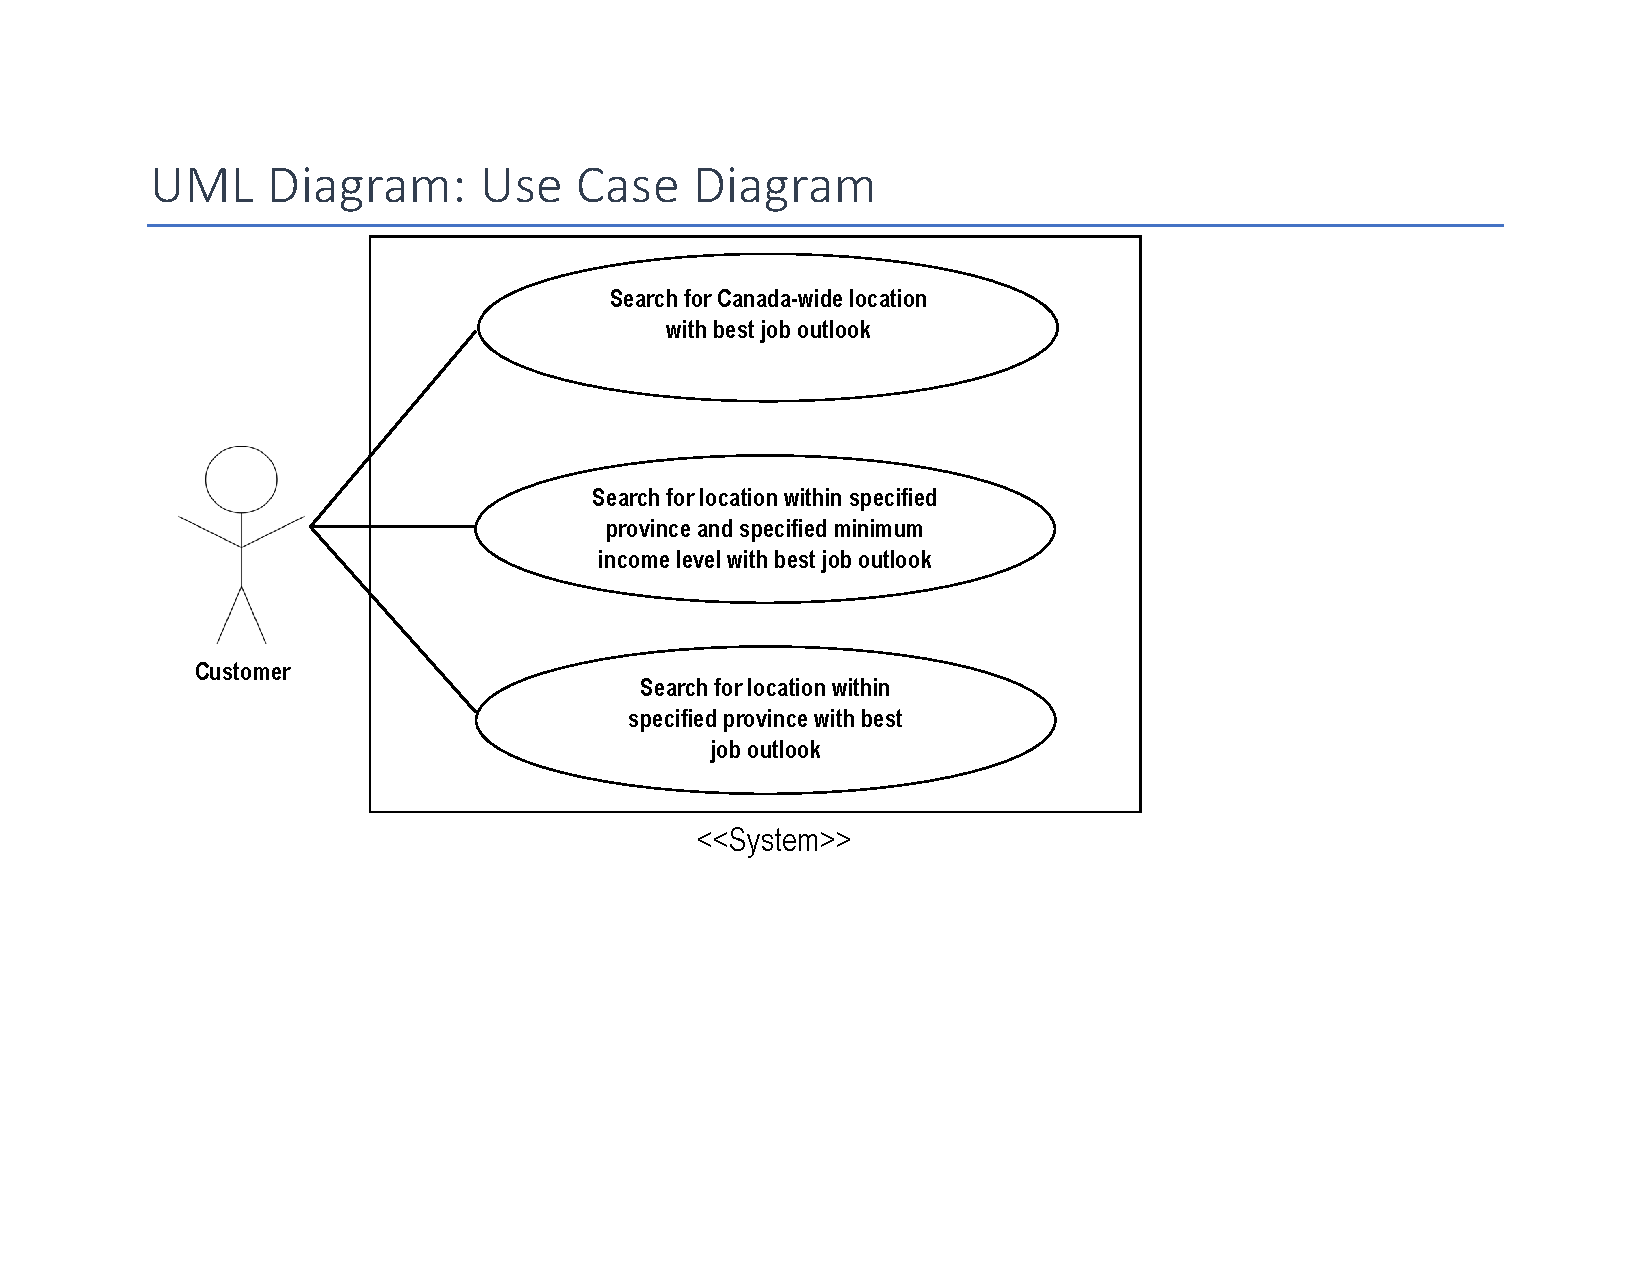
\includegraphics[width=\linewidth] {Group04_Uses_Diagram.pdf}
  \caption{Uses Case Diagram for ReLocate product.}
  \label{fig:uses}
\end{figure}




%%%%%%%%%%%%%%%%%%%%%%%%%%%%%%%%%%%%%%%%%%%%%%%%%%%%%%%%%%%%%%%%%%%%%%

\newpage
\section*{Traceability Matrix}

%%%%%%%%%%%%%%%%%%%%%%%%%%%%%%%%%%%%%%%%%%%%%%%%%%%%%%%%%%%%%%%%%%%%%%

\newpage

\section*{Private Methods Description}
\subsection*{City.java}\label{pcity}

\subsubsection*{Semantics}
\subsubsection*{State (Instance) Variables}
	private final String $cityName$\\
	private Province $province$\\
	private Outlook $cityOutlook$\\
	private double $income$
\subsubsection*{Access Routine Semantics}


\subsection*{CityData.java}\label{pcityd}

\subsubsection*{Semantics}
\subsubsection*{State (Instance) Variables}
	private final int $year$\\
	private final String $city$\\
	private final String $province$\\
	private final String $GeographicalID$\\
	private final String $DataType$\\
	private final String $Vector$\\
	private final double $Coordinate$\\
	private final double $Income$
\subsubsection*{Access Routine Semantics}


\subsection*{CityGraph.java}\label{pgraph}
\subsubsection* {Syntax}

\subsubsection* {Access Programs}
\begin{tabular}{| l | l | l | l |}
\hline
\textbf{Routine name} & \textbf{Input} & \textbf{Output} & \textbf{Exceptions}\\
\hline
~ & ~ & ~ & ~\\
\hline
\end{tabular}

\subsubsection*{Semantics}
\subsubsection*{State (Instance) Variables}
	private final double $SCALING\_FACTOR$ = 1\\
	private final int $CITIES\_TO\_RETURN$ = 2\\
	private ArrayList$<$GraphVertex$>$ $vertices$
\subsubsection*{Access Routine Semantics}


\subsection*{CityIncome.java}\label{pcityincome}

\subsubsection*{Semantics}
\subsubsection*{State (Instance) Variables}
	private final String $cityName$\\
	private String $province$\\
	private ArrayList$<$Double$>$ $incomes$\\
	private double $avgIncome$
\subsubsection*{Access Routine Semantics}


\subsection*{GraphEdge.java}\label{pedge}

\subsubsection*{Semantics}
\subsubsection*{State (Instance) Variables}
	private GraphVertex $v$\\
	private GraphVertex $w$\\
	private long $weight$
\subsubsection*{Access Routine Semantics}


\subsection*{GraphVertex.java}\label{pvertex}

\subsubsection*{Semantics}
\subsubsection*{State (Instance) Variables}
	private City $city$\\
	private double $outlook$\\
	private ArrayList$<$GraphEdge$>$ $adj$
\subsubsection*{Access Routine Semantics}


\subsection*{Income.java}\label{pincome}


\subsubsection*{Semantics}
\subsubsection*{State (Instance) Variables}
ArrayList$<$CityIncome$>$ $cities$
\subsubsection*{Access Routine Semantics}


\subsection*{Job.java}\label{pjob}

\subsubsection*{Semantics}
\subsubsection*{State (Instance) Variables}
	private final String $name$\\
	private ArrayList$<$Province$>$ $provinces$

\subsubsection*{Access Routine Semantics}


\subsection*{JobArray.java}\label{pjobarray}

\subsubsection*{Semantics}
\subsubsection*{State (Instance) Variables}
    	ArrayList$<$Job$>$ $jobs$\\
	Income $incomeFetcher$\\
	ArrayList$<$CityIncome$>$ $income$\\
	ProvinceMap $map$
\subsubsection*{Access Routine Semantics}


\subsection*{MergeSort.java}\label{psort}
\subsubsection* {Syntax}

\subsubsection* {Access Programs}
\begin{tabular}{| l | l | l | l |}
\hline
\textbf{Routine name} & \textbf{Input} & \textbf{Output} & \textbf{Exceptions}\\
\hline
~ & ~ & ~ & ~\\
\hline
~ & ~ & ~ & ~\\
\hline
\end{tabular}

\subsubsection*{Semantics}
\subsubsection*{State (Instance) Variables}
	private static ArrayList$<$Comparable$>$ $aux$
\subsubsection*{Access Routine Semantics}


\subsection*{Outlook.java}\label{poutlook}

\subsubsection*{Semantics}
\subsubsection*{State (Instance) Variables}
	private int $potential$\\
	private String $trend$\\
	private City $city$
\subsubsection*{Access Routine Semantics}


\subsection*{OutlookData.java}\label{poutlookd}

\subsubsection*{Semantics}
\subsubsection*{State (Instance) Variables}
	private final String $Title,CPP,Trends,TrendsDate,Lang,ProvAbbr,Location$\\
	private final int $potential,code,provID, NOC, cityID$
\subsubsection*{Access Routine Semantics}


\subsection*{Parser.java}\label{pparser}
\subsubsection* {Syntax}

\subsubsection* {Access Programs}
\begin{tabular}{| l | l | l | l |}
\hline
\textbf{Routine name} & \textbf{Input} & \textbf{Output} & \textbf{Exceptions}\\
\hline
~ & ~ & ~ & ~\\
\hline
\end{tabular}

\subsubsection*{Semantics}
\subsubsection*{State (Instance) Variables}
	private final String $outlookName$ = "data/outlooks.csv"\\
	private final String $incomeName$ = "data/income.csv"
\subsubsection*{Access Routine Semantics}


\subsection*{Province.java}\label{pprov}

\subsubsection*{Semantics}
\subsubsection*{State (Instance) Variables}
	private final String $provinceCode$\\
	private double $avgPotential$\\
	private double $provinceIncome$\\
	private Job $job$\\
	private ArrayList$<$City$>$ $cities$\\
	private ArrayList$<$String$>$ $provinceTrends$\\
\subsubsection*{Access Routine Semantics}


\subsection*{ProvinceMap.java}\label{pprovmap}

\subsubsection*{Semantics}
\subsubsection*{State (Instance) Variables}
	private final String $f$ = "data/provinces.txt"\\
	private Map$<$String,String$>$ $forward$ = new Hashtable$<$String,String$>$()\\
	private Map$<$String,String$>$ $backward$ = new Hashtable$<$String,String$>$()
\subsubsection*{Access Routine Semantics}


\subsection*{Searcher.java}\label{psearch}

\subsubsection*{Semantics}
\subsubsection*{State (Instance) Variables}
\subsubsection*{Access Routine Semantics}
		JobArray $jobsFetcher$\\
		ArrayList$<$Job$>$ $ jobs$


%%%%%%%%%%%%%%%%%%%%%%%%%%%%%%%%%%%%%%%%%%%%%%%%%%%%%%%%%%%%%%%%%%%%%%

\newpage
\section*{Review of Design}


\end{document}